% \documentclass[../../main.tex]{subfiles}

% \begin{document}

% \section{Dmytruk and Schir\'o (2021): gauge fixing for correlated electrons
% coupled to quantum light}
% \label{sec:dmytruk2021}

% \subsection*{Source}
% O.~Dmytruk and M.~Schir\'o, \emph{Gauge fixing for strongly correlated electrons
% coupled to quantum light}, Phys.\ Rev.\ B \textbf{103}, 075131 (2021).
% Equations are cited as Eq.~(n) with the paper's numbering; appendix equations as
% Eq.~(A.n).

\documentclass[11pt]{article}

\usepackage[margin=24mm]{geometry}
\usepackage[T1]{fontenc}
\usepackage{lmodern}
\usepackage{amsmath,amssymb}
\usepackage{xcolor}
\usepackage{cancel}
\usepackage{tikz}
\usepackage{cleveref}

\allowdisplaybreaks[2]
\setlength{\parindent}{0pt}
\setlength{\parskip}{4pt}

% The orange references in the scan give the source's equation numbers.
% Register those numbers separately from the equations numbered in these notes.
\makeatletter
\newcommand{\externalequation}[3]{%
  \newlabel{#1}{{#3}{}{}{}{}}%
  \newlabel{#1@cref}{{[equation][#2][]#3}{}{}{}{}}%
}
\makeatother
\newcommand{\paperref}[1]{\textcolor{orange}{\labelcref{#1}}}
\newcommand{\stepref}[1]{\overset{\text{\scriptsize\labelcref{#1}}}{=}}
\newcommand{\annotation}[1]{\textcolor{violet}{#1}}
\newcommand{\crossout}[1]{{\renewcommand{\CancelColor}{\color{violet}}\cancel{#1}}}
\newcommand{\done}{\mathrel{/\mkern-5mu/}}
\newcommand{\dint}{\mathop{}\!\mathrm{d}}
\newcommand{\highlight}[2]{\colorbox{#1!30}{\strut #2}}

\externalequation{paper:1}{1}{1}
\externalequation{paper:2}{2}{2}
\externalequation{paper:3}{3}{3}
\externalequation{paper:4}{4}{4}
\externalequation{paper:6}{6}{6}
\externalequation{paper:7}{7}{7}
\externalequation{paper:9}{9}{9}
\externalequation{paper:13}{13}{13}
\externalequation{paper:14}{14}{14}
\externalequation{paper:15}{15}{15}
\externalequation{paper:21}{21}{21}
\externalequation{paper:23}{23}{23}
\externalequation{paper:27}{27}{27}
\externalequation{paper:28}{28}{28}
\externalequation{paper:29}{29}{29}
\externalequation{paper:31}{31}{31}
\externalequation{paper:33}{33}{33}
\externalequation{paper:34}{34}{34}
\externalequation{paper:37}{37}{37}
\externalequation{paper:38}{38}{38}
\externalequation{paper:44}{44}{44}
\externalequation{paper:A.1}{1}{A.1}
\externalequation{dutra:2.110}{110}{2.110}
\externalequation{dutra:2.111}{111}{2.111}

\begin{document}

% Source page 1
\section*{\colorbox{magenta!30}{\parbox{\dimexpr\linewidth-2\fboxsep\relax}{Gauge fixing for strongly correlated electrons coupled to quantum light \textasciitilde{} Schiro}}}

\begin{align*}
H_{\mathrm{el}}
  &= \int \dint r\,\psi^\dagger(r)
     \left(-\frac{\nabla^2}{2m}+V(r)\right)\psi(r)\\
  &\quad + \int \dint r\,\dint r'\,
     \psi^\dagger(r)\psi^\dagger(r')U(r-r')\psi(r')\psi(r)
     \qquad \paperref{paper:1,paper:2,paper:3}\\
  &\Rightarrow \text{invariant under}\quad
     \psi(r)\to e^{i\chi}\psi(r).
\end{align*}


\begin{align*}
H_{\mathrm{el}}&=H_{\mathrm{el}}(\psi,\psi^\dagger)
  \qquad \& \qquad
  H(\vec p,\vec q,t)=\sum_{i=1}^{n}p_i\dot{\vec q}^{\,i}
    -L(\vec q,\dot{\vec q},t) \qquad \text{(wiki)}
\end{align*}
\begin{equation}
\Rightarrow\quad L_{\mathrm{el}}(\psi,\psi^\dagger)
  =\int \dint r\,\psi^\dagger(r)(\partial_t\psi(r))-H_{\mathrm{el}}.
\label{eq:electron-lagrangian}
\end{equation}
\[
\Rightarrow \text{invariant under}\quad
 \psi(r)\to e^{i\chi}\psi(r)
 \qquad \& \qquad L_{\mathrm{el}}=\int \dint r\,\mathcal L_{\mathrm{el}}.
\]

 Peskin: For
\begin{gather*}
\phi(x)\to\phi'(x)=\phi(x)+\alpha\Delta\phi(x)
\quad \&\quad
\mathcal L(x)\to\mathcal L(x)+\alpha\partial_\mu J^\mu(x),\\
\partial_\mu j^\mu(x)=0
\quad \text{for}\quad
j^\mu(x)=\frac{\partial\mathcal L}{\partial(\partial_\mu\phi)}
          \Delta\phi-J^\mu.
\end{gather*}

 Our trafo can be infinitesimally be written as
\[
\psi\to\psi+i\chi\psi
\quad \underline{\text{and}}\quad
\psi^\dagger\to\psi^\dagger-i\chi\psi^\dagger,
\quad \text{with \(\chi\) small}.
\]

 Since \(\mathcal L_{\mathrm{el}}\to\mathcal L_{\mathrm{el}}\), we can set \(J^\mu(x)=0\)
\begin{align*}
\Rightarrow\quad j^\mu(x)
  &=\frac{\partial\mathcal L}{\partial(\partial_\mu\psi)}
     \cdot(i\psi)
    +\frac{\partial\mathcal L}{\partial(\partial_\mu\psi^\dagger)}
     \cdot(-i\psi^\dagger)\\
j^0(r)&\stepref{eq:electron-lagrangian}\psi^\dagger(r)\cdot(i\psi(r)).
\end{align*}

 For the other components, only first term of \(H_{\mathrm{el}}\) (\(H_0\)) is relevant

Rewrite:
\begin{align*}
H_{0,\mathrm{kin}}
  &=\int \dint r\,\psi^\dagger(r)
        \left(-\frac{\nabla^2}{2m}\right)\psi(r)\\
  &\overset{\mathrm{P.I.}}{=}
    \left.\psi^\dagger(r)\left(-\frac{\nabla}{2m}\right)\psi(r)\right|_\Omega
    +\frac{1}{2m}\int \dint r\,(\nabla\psi^\dagger(r))(\nabla\psi(r))\\
  &=\frac{1}{2m}\int \dint r\,(\nabla\psi^\dagger(r))(\nabla\psi(r))
    \qquad \text{with \(\psi=0\) at inf.}
\end{align*}

% Source page 2
\begin{align*}
\Rightarrow\quad \vec j(r)
 &=\frac{\partial\mathcal L_{\mathrm{el}}}{\partial(\nabla\psi)}\cdot(i\psi)
   -\frac{\partial\mathcal L_{\mathrm{el}}}{\partial(\nabla\psi^\dagger)}
     (i\psi^\dagger)\\
 &=\frac{i}{2m}\left\{(\nabla\psi^\dagger(r))\psi
       -\overbrace{(\nabla\psi(r))}^{\annotation{\text{field op.}}}
           \psi^\dagger(r)\right\}
   \quad\done\quad \paperref{paper:4}
   \quad \text{missing factor of \(2\)}
\end{align*}

 Eqs. \paperref{paper:6,paper:7} roughly from
\textcolor{orange}{\crefrange{dutra:2.110}{dutra:2.111}} of Dutra \annotation{?}


\[
\mathcal U(\chi)=\exp\left[i(a+a^\dagger)
      \int \dint r\,\psi^\dagger(r)\chi(r)\psi(r)\right],
\quad \text{\(\chi(r)\) is a real function}.
\]
\begin{align*}
\text{claim:}\quad
\mathcal U^\dagger\psi(r)\mathcal U
  &=e^{i(a+a^\dagger)\chi(r)}\psi(r)
       \qquad \text{w.}\quad
       \mathcal U^\dagger\mathcal U=\mathcal U\mathcal U^\dagger=\mathbb 1\\
\Rightarrow\quad\mathcal U^\dagger\psi(r)
  &=e^{i(a+a^\dagger)\chi(r)}\psi(r)\mathcal U^\dagger\\
\psi(r)\mathcal U
  &=\psi(r)\sum_{n=0}^{\infty}\frac{(i)^n}{n!}(a+a^\dagger)^n
     \left(\int \dint r'\,\psi^\dagger(r')\chi(r')\psi(r')\right)^n
\end{align*}
with \([\psi(r),a^{(\dagger)}]=0\)
\quad \& \quad \(\{\psi(r),\psi^\dagger(r')\}=\delta(r-r')\)

and \(\{\psi(r),\psi(r')\}=0\) follows
\begin{align}
&\psi(r)\left(\int \dint r'\,\psi^\dagger(r')\chi(r')\psi(r')\right)
   \notag\\
&\qquad=\int \dint r'\,
  \left(\delta(r-r')-\psi^\dagger(r')\psi(r)\right)\chi(r')\psi(r')
   \notag\\
&\qquad=\chi(r)\psi(r)
  +\left(\int \dint r'\,\psi^\dagger(r')\chi(r')\psi(r')\right)\psi(r).
\label{eq:commute-field-once}
\end{align}
With \(I\equiv\int \dint r'\,\psi^\dagger(r')\chi(r')\psi(r')\),
\cref{eq:commute-field-once} reads
\[
\psi(r)I=\chi(r)\psi(r)+I\psi(r)
\quad\Leftrightarrow\quad [\psi(r),I]=\chi(r)\psi(r).
\]
\begin{align}
\Rightarrow\quad\psi(r)II
  &=\psi(r)\left(\int \dint r'\,\psi^\dagger(r')\chi(r')\psi(r')\right)^2
    \notag\\
  &\stepref{eq:commute-field-once}\chi(r)\psi(r)I+I\psi(r)I
    \notag\\
  &\stepref{eq:commute-field-once}
       \chi^2(r)\psi(r)+\chi(r)I\psi(r)+\chi(r)I\psi(r)+I^2\psi(r)
    \notag\\
  &=\chi^2(r)\psi(r)+2\chi(r)I\psi(r)+I^2\psi(r)
    \notag\\
  &=(\chi(r)+I)^2\psi(r).
\label{eq:commute-field-twice}
\end{align}

% Source page 3
\begin{align*}
&\psi(r)\left(\int \dint r'\,\psi^\dagger(r')\chi(r')\psi(r')\right)^3\\
&\qquad=\psi(r)
  \left(\int \dint r'\,\psi^\dagger(r')\chi(r')\psi(r')\right)
  \left(\int \dint r'\,\psi^\dagger(r')\chi(r')\psi(r')\right)^2\\
&\qquad\stepref{eq:commute-field-once}(\chi(r)+I)\psi(r)I^2\\
&\qquad\stepref{eq:commute-field-twice}(\chi(r)+I)^3\psi(r)
\end{align*}
\begin{equation}
\cdots\ \Rightarrow\quad\psi(r)I^n=(\chi(r)+I)^n\psi(r)
\qquad \done
\label{eq:commute-field-power}
\end{equation}
\begin{align*}
\Rightarrow\quad\psi(r)\mathcal U
  &=\psi(r)\sum_{n=0}^{\infty}\frac{(i)^n}{n!}(a+a^\dagger)^n
     \left(\int \dint r'\,\psi^\dagger(r')\chi(r')\psi(r')\right)^n\\
  &\overset{\annotation{[\psi,a^{(\dagger)}]=0}}{=}
     \sum_{n=0}^{\infty}\frac{(i)^n}{n!}(a+a^\dagger)^n\psi(r)
     \left(\int \dint r'\,\psi^\dagger(r')\chi(r')\psi(r')\right)^n\\
  &\stepref{eq:commute-field-power}
     \sum_{n=0}^{\infty}\frac{(i)^n}{n!}(a+a^\dagger)^n
     \left(\chi(r)+\int \dint r'\,\psi^\dagger(r')\chi(r')\psi(r')\right)^n
        \psi(r)\\
  &=\exp\left\{i(a+a^\dagger)
       \left(\chi(r)+\int \dint r'\,\psi^\dagger(r')\chi(r')\psi(r')\right)
     \right\}\psi(r)\\
  &\overset{\annotation{\substack{[\psi,a^{(\dagger)}]=0\\\text{BCH}}}}{=}
       \mathcal U\exp\left(i(a+a^\dagger)\chi(r)\right)\psi(r)\\
\Rightarrow\quad\mathcal U^\dagger\psi(r)\mathcal U
  &=e^{i(a+a^\dagger)\chi(r)}\psi(r)\qquad\done
     \qquad\paperref{paper:13}\;\textcolor{orange}{\downarrow}
\end{align*}

 Furthermore, with \([a,a^\dagger]=1\) (single mode) follows
\begin{align*}
\hat n(\hat a+\hat a^\dagger)
  &=a^\dagger a(a+a^\dagger)=a^\dagger aa+a^\dagger aa^\dagger\\
  &=(aa^\dagger-1)a+a^\dagger(1+a^\dagger a)\\
  &=an-a+a^\dagger+a^\dagger n\\
  &=a^\dagger-a+(a+a^\dagger)n\\
\Rightarrow\quad[n,a+a^\dagger]&=a^\dagger-a
\end{align*}

 Write \(S=(a+a^\dagger)\int \dint r\,\psi^\dagger(r)\chi(r)\psi(r)\)
\qquad \paperref{paper:A.1}
\begin{align*}
\mathcal U H_{\mathrm{ph}}\mathcal U^\dagger
 &=e^{iS}H_{\mathrm{ph}}e^{-iS}
 \overset{\annotation{\text{BCH}}}{=} H_{\mathrm{ph}}+[iS,H_{\mathrm{ph}}]
    +\frac{1}{2!}[iS,[iS,H_{\mathrm{ph}}]]+\cdots
\end{align*}

% Source page 4
with \([iS,H_{\mathrm{ph}}]=i(a-a^\dagger)I\omega_c\) follows
\begin{align*}
[a+a^\dagger,i(a-a^\dagger)I]
  &=\bigl(i\overbrace{[a,a]}^{\annotation{0}}-i[a,a^\dagger]
       +i[a^\dagger,a]-i\overbrace{[a^\dagger,a^\dagger]}^{\annotation{0}}
      \bigr)I\omega_c\\
  &=\bigl(-2i[a,a^\dagger]\bigr)I=-2iI\omega_c\quad\text{and}\\
[iS,[iS,H_{\mathrm{ph}}]]
  &=[iS,i(a-a^\dagger)I]\\
  &=2I^2\omega_c\\
\Rightarrow\quad[iS,[iS,[iS,H_{\mathrm{ph}}]]]
  &=[iS,2I]=0
\end{align*}
\begin{equation}
\Rightarrow\quad\mathcal U H_{\mathrm{ph}}\mathcal U^\dagger
 =H_{\mathrm{ph}}+i\omega_c(a-a^\dagger)I+2\omega_c I^2
 \ne H_{\mathrm{ph}}.
\label{eq:transformed-photons}
\end{equation}
\[
\Rightarrow \text{in eq \paperref{paper:15} only the el.\ part is transformed}
\qquad\done
\]

 \cref{eq:transformed-photons} actually leads to \paperref{paper:21}
\quad \annotation{(additional factor of \(2\))}

 Since
\(\mathcal U^\dagger\psi^{(\dagger)}(r)\mathcal U
 =e^{\pm i(a+a^\dagger)\chi(r)}\psi^{(\dagger)}\)
it directly follows that
\(\mathcal U^\dagger H_{\mathrm{ee}}\mathcal U=H_{\mathrm{ee}}\)

 giv.:
\begin{gather*}
H_0=\int \dint r\,\psi^\dagger(r)
    \left(-\frac{\nabla^2}{2m}+V(r)\right)\psi(r),
\qquad
\mathcal U^\dagger\psi(r)\mathcal U=e^{i(a+a^\dagger)\chi(r)}\psi(r)\\
\mathcal U^\dagger\psi^\dagger(r)\mathcal U
   =\psi^\dagger(r)e^{-i(a+a^\dagger)\chi(r)}
\end{gather*}
\begin{align*}
\Rightarrow\quad\mathcal U^\dagger H_{0,\mathrm{pot}}\mathcal U
 &=\int \dint r\,
   \mathcal U^\dagger\psi^\dagger(r)
   \underbrace{\overbrace{\mathcal U\mathcal U^\dagger}^{\annotation{=1}}
       V(r)\overbrace{\mathcal U\mathcal U^\dagger}^{\annotation{=1}}}
       _{\annotation{=V(r)}}\psi(r)\mathcal U\\
 &=\int \dint r\,\psi^\dagger(r)\crossout{e^{-i(a+a^\dagger)\chi(r)}}
       V(r)\crossout{e^{i(a+a^\dagger)\chi(r)}}\psi(r)\\
 &=H_{0,\mathrm{pot}}\qquad\done
\end{align*}
Use again
\[
H_{0,\mathrm{kin}}
  =\frac{1}{2m}\int \dint r\,(\nabla\psi^\dagger(r))(\nabla\psi(r))
  =-\frac{1}{2m}\int \dint r\,\psi^\dagger(r)\nabla^2\psi(r).
\]

% Source page 5
\begin{align*}
\mathcal U^\dagger H_{0,\mathrm{kin}}\mathcal U
 &=\frac{-1}{2m}\int \dint r\,
    \mathcal U^\dagger\psi^\dagger(r)\mathcal U\mathcal U^\dagger
     \nabla^2\mathcal U\mathcal U^\dagger\psi(r)\mathcal U\\
 &=\frac{-1}{2m}\int \dint r\,\psi^\dagger(r)e^{-i(a+a^\dagger)\chi(r)}
    \underbrace{\mathcal U^\dagger\nabla^2\bigl(
      \overbrace{\mathcal U}^{\annotation{\text{indep. of \(r\)}}}}
      _{\annotation{1}}
      e^{i(a+a^\dagger)\chi(r)}\psi(r)\bigr)\\
 &=\frac{-1}{2m}\int \dint r\,\psi^\dagger(r)e^{-i(a+a^\dagger)\chi(r)}
      \nabla^2\bigl(e^{i(a+a^\dagger)\chi(r)}\psi(r)\bigr)
\end{align*}
\begin{align*}
\nabla^2\bigl(e^{i(a+a^\dagger)\chi(r)}\psi(r)\bigr)
 &=\nabla\left\{\bigl(\nabla e^{i(a+a^\dagger)\chi(r)}\bigr)\psi(r)
   +e^{i(a+a^\dagger)\chi(r)}(\nabla\psi(r))\right\}\\
 &=\bigl(\nabla^2 e^{i(a+a^\dagger)\chi(r)}\bigr)\psi(r)
    +2\bigl(\nabla e^{i(a+a^\dagger)\chi(r)}\bigr)(\nabla\psi(r))\\
 &\quad +e^{i(a+a^\dagger)\chi(r)}(\nabla^2\psi(r))
\end{align*}
\begin{align*}
\text{with}\quad \nabla e^{i(a+a^\dagger)\chi(r)}
  &=(\nabla\chi(r))i(a+a^\dagger)e^{i(a+a^\dagger)\chi(r)}
    \qquad \text{and}\\
\nabla^2e^{i(a+a^\dagger)\chi(r)}
  &=\left\{(\nabla^2\chi(r))i(a+a^\dagger)
     -(a+a^\dagger)^2(\nabla\chi(r))^2\right\}
       e^{i(a+a^\dagger)\chi(r)}
\end{align*}
\begin{align*}
&\Rightarrow\quad\nabla^2\bigl(e^{i(a+a^\dagger)\chi(r)}\psi(r)\bigr)\\
&\quad=
 \Bigl\{
   i\underbrace{(a+a^\dagger)
      \overbrace{\nabla^2\chi(r)}^{\annotation{=\nabla e A_0(r)}}}
      _{\annotation{=e\nabla A(r)}}\psi(r)
   -\underbrace{(a+a^\dagger)^2
      \overbrace{(\nabla\chi(r))^2}^{\annotation{=e^2 A_0^2(r)}}}
      _{\annotation{=e^2 A^2(r)}}\psi(r)\\
&\qquad\quad +2i\underbrace{(a+a^\dagger)(\nabla\chi(r))}
       _{\annotation{=eA(r)}}(\nabla\psi(r))
   +\nabla^2\psi(r)
 \Bigr\}e^{i(a+a^\dagger)\chi(r)}\\[2pt]
&\quad\overset{\substack{\text{\scriptsize\paperref{paper:14}}\\
       \annotation{\nabla\chi(r)=eA_0(r)}\\
       \annotation{A(r)=A_0(r)\times(a+a^\dagger)}}}{=}
    \bigl\{ie\nabla A(r)\psi(r)-e^2A^2(r)\psi(r)
      +2ieA(r)\nabla\psi(r)+\nabla^2\psi(r)\bigr\}
      e^{i(a+a^\dagger)\chi(r)}\\
&\quad=\bigl\{(-i\nabla+eA)^2\psi(r)+ieA(r)\nabla\psi(r)\bigr\}
      e^{i(a+a^\dagger)\chi(r)}
\end{align*}
\begin{align*}
\Rightarrow\quad \mathcal U^\dagger H_{0,\mathrm{kin}}\mathcal U
  &=\frac{-1}{2m}\int \dint r\,\psi^\dagger(r)
       \crossout{e^{-i(a+a^\dagger)\chi(r)}}\crossout{e^{i(a+a^\dagger)\chi(r)}}\\
  &\qquad{}\times
    \bigl\{(-i\nabla+eA)^2\psi(r)+ieA(r)\nabla\psi(r)\bigr\}\\
  &=\frac{-1}{2m}\int \dint r\,\psi^\dagger(r)(-i\nabla+eA(r))^2\psi(r)
      \quad \textcolor{red}{\Rightarrow \text{minimal coupling}}\\
  &\qquad{}-\frac{ie}{2m}\int \dint r\,\psi^\dagger(r)A(r)\nabla\psi(r).
\end{align*}

% Source page 6
\begin{align*}
\Rightarrow\quad\widetilde H_C
 &=H_{\mathrm{ph}}+\mathcal U^\dagger(H_0+H_{\mathrm{ee}})\mathcal U
   =H_{\mathrm{ph}}+H_{\mathrm{ee}}+\mathcal U^\dagger H_0\mathcal U\\
 &=H_{\mathrm{ph}}+H_{\mathrm{ee}}+\int \dint r\,
      \psi^\dagger(r)h_C(r)\psi(r)\\
 &\quad -\frac{ie}{2m}\int \dint r\,\psi^\dagger(r)A(r)\nabla\psi(r)
\end{align*}
\begin{align*}
-\frac{ie}{2m}\int \dint r\,\psi^\dagger(r)A(r)\nabla\psi(r)
 &\overset{\annotation{\substack{\text{P.I.}\\
         \text{\& \(\psi=0\) on boundary}}}}{=}
    \frac{ie}{2m}\int \dint r\,\psi^\dagger(r)\nabla A(r)\psi(r)\\
 &=0\qquad \text{for Coulomb gauge}
\end{align*}
\begin{align*}
\Rightarrow\quad H_C
 &=H_{\mathrm{ph}}+\mathcal U^\dagger(H_0+H_{\mathrm{ee}})\mathcal U\\
 &=H_{\mathrm{ph}}+H_{\mathrm{ee}}+\int \dint r\,\psi^\dagger(r)h_C(r)\psi(r)
 \qquad\done\qquad\textcolor{orange}{\downarrow}\,
   \paperref{paper:14}\ \paperref{paper:9}
\end{align*}

\highlight{orange}{Summary:} Interaction between matter (els.) and the em field
can be either introduced via
\begin{enumerate}
\renewcommand{\labelenumi}{\roman{enumi})}
\item Minimal coupling: \(-i\nabla\to-i\nabla+eA(r)\) or
\item Performing a unitary trafo on the matter d.o.f.
\begin{quote}
\(\hookrightarrow\) System is inv. under global phase trafo
\(\psi\to e^{i\chi(r)}\psi(r)\)

\(\qquad\Leftrightarrow\) current is conserved

\(\hookrightarrow\) promote this global, to a local trafo, i.e.,
\[
\psi(r)\to e^{i\chi(r)}\psi(r)=\mathcal U^\dagger\psi(r)\mathcal U
\]
\end{quote}
\end{enumerate}

\hrule


 Project \(\mathcal U\) by \(U=P\mathcal U P\) where
\[
\mathcal U=\exp\left[i(a+a^\dagger)
 \overbrace{\int \dint r\,\psi^\dagger(r)\chi(r)\psi(r)}^{\annotation{=S}}\right]
 \qquad \paperref{paper:13}
\]

% Source page 7
and
\[
P\psi^{(\dagger)}(r)P
  =\Psi^{(\dagger)}(r)=\sum_{R,\mu}\phi^{(*)}_{R\mu}(r)c^{(\dagger)}_{R\mu}
  \qquad \paperref{paper:23}
\]

 Note, that we only want to project the \underline{electronic} part
onto a subspace (e.g. few bands around Fermi energy)
\[
\hookrightarrow\quad PaP=a\qquad\&\qquad Pa^\dagger P=a^\dagger
\]


\begin{align*}
PSP\mathrel{\textcolor{red}{\ne}}
  \int \dint r\sum_{R,R',\mu,\mu'}
    \phi^*_{R\mu}(r)\chi(r)c^\dagger_{R\mu}
    \phi_{R'\mu'}(r)c_{R'\mu'}
   &=\overbrace{\sum_{R,R',\mu,\mu'}
       \chi_{RR'}^{\mu\mu'}c^\dagger_{R\mu}c_{R'\mu'}}
       ^{\annotation{S_p}}
     \qquad \paperref{paper:27,paper:28}
\end{align*}
\textcolor{red}{by \(PSP\), apparently is meant to simply to}
\[
\textcolor{red}{
S(\psi,\psi^\dagger)\to S\bigl(\textstyle\sum\phi c,
                              \textstyle\sum\phi^*c^\dagger\bigr)}
\]
\(\Rightarrow\) term missing, that would actually result from \(P\cdot P\)

 Campbell identity:
\begin{equation}
e^X Y e^{-X}=\sum_{n=0}^\infty\frac{[X,Y]_n}{n!}
\label{eq:campbell}
\end{equation}
with
\[
[X,Y]_n=[X,\ldots[X,Y]\ldots]
\qquad\&\qquad [X,Y]_0\equiv Y
\]


\begin{align*}
U(\chi)
 &=\exp\left(i(a+a^\dagger)\sum_{RR'}\sum_{\mu\mu'}
         c^\dagger_{R\mu}\chi_{RR'}^{\mu\mu'}c_{R'\mu'}\right)\\
 &=e^{-iS}\\
\hookrightarrow\quad U^\dagger(\chi)
 &=\exp\left(-i(a^\dagger+a)\sum_{RR'}\sum_{\mu\mu'}
       c^\dagger_{R'\mu'}\chi_{R'R}^{\mu'\mu}c_{R\mu}\right)
       \qquad \annotation{[a^{(\dagger)},c^{(\dagger)}]=0}\\
 &=\exp\left(-i(a+a^\dagger)\sum_{RR'}\sum_{\mu\mu'}
       c^\dagger_{R\mu}\chi_{RR'}^{\mu\mu'}c_{R'\mu'}\right)\\
 &=e^{iS}\qquad\Rightarrow\quad U^\dagger U=UU^\dagger=\mathbb 1\\
\Rightarrow\quad U^\dagger c_{R\mu}U
 &=e^{iS}c_{R\mu}e^{-iS}\\
 &\stepref{eq:campbell}\sum_{n=0}^\infty\frac{[iS,c_{R\mu}]_n}{n!}
\end{align*}

% Source page 8

\begin{align*}
-c_{R\mu}iS
 &=ic_{R\mu}(a+a^\dagger)\sum_{R'R''}\sum_{\mu'\mu''}
      c^\dagger_{R'\mu'}\chi_{R'R''}^{\mu'\mu''}c_{R''\mu''}\\
 &\overset{\annotation{\{c_\alpha,c_\beta^\dagger\}=\delta_{\alpha\beta}}}{=}
    i(a+a^\dagger)\sum_{R'R''}\sum_{\mu'\mu''}\chi_{R'R''}^{\mu'\mu''}
       \left(\delta_{RR'}\delta_{\mu\mu'}c_{R''\mu''}
           -c^\dagger_{R'\mu'}c_{R\mu}c_{R''\mu''}\right)\\
 &=i(a+a^\dagger)\sum_{R''}\sum_{\mu''}\chi_{RR''}^{\mu\mu''}c_{R''\mu''}\\
 &\quad+i(a+a^\dagger)\sum_{R'R''}\sum_{\mu'\mu''}
     \chi_{R'R''}^{\mu'\mu''}c^\dagger_{R'\mu'}c_{R''\mu''}c_{R\mu}\\
 &=i(a+a^\dagger)\sum_{R'\mu'}\chi_{RR'}^{\mu\mu'}c_{R'\mu'}-iS c_{R\mu}
\end{align*}
\begin{equation}
\Rightarrow\quad[iS,c_{R\mu}]
  =i(a+a^\dagger)\sum_{R'\mu'}\chi_{RR'}^{\mu\mu'}c_{R'\mu'}
  \qquad\done
\label{eq:lattice-first-commutator}
\end{equation}
\begin{align}
\Rightarrow\quad[iS,[iS,c_{R\mu}]]
 &\stepref{eq:lattice-first-commutator}
   \left[iS,i(a+a^\dagger)\sum_{R'\mu'}\chi_{RR'}^{\mu\mu'}c_{R'\mu'}\right]
   \notag\\
 &\overset{\annotation{\substack{[a+a^\dagger,a+a^\dagger]\\=0=[A,A]}}}{=}
      i(a+a^\dagger)\sum_{R'\mu'}\chi_{RR'}^{\mu\mu'}[iS,c_{R'\mu'}]
   \notag\\
 &\stepref{eq:lattice-first-commutator}
      [i(a+a^\dagger)]^2\sum_{R'\mu'}\chi_{RR'}^{\mu\mu'}
          \sum_{R''\mu''}\chi_{R'R''}^{\mu'\mu''}c_{R''\mu''}
   \label{eq:lattice-second-commutator}\\
 &\overset{\text{\highlight{magenta}{(?)}}}{=}
      [i(a+a^\dagger)]^3\sum_{R'\mu'}(\chi_{RR'}^{\mu\mu'})^2c_{R'\mu'}
   \notag
\end{align}
\begin{align*}
&\Rightarrow\quad[iS,[iS,[iS,c_{R\mu}]]]\\
&\qquad\stepref{eq:lattice-second-commutator}
    \left[iS,[i(a+a^\dagger)]^2
       \sum_{R'\mu'}\chi_{RR'}^{\mu\mu'}
       \sum_{R''\mu''}\chi_{R'R''}^{\mu'\mu''}c_{R''\mu''}\right]\\
&\qquad=[i(a+a^\dagger)]^2\sum_{R'\mu'R''\mu''}
       \chi_{RR'}^{\mu\mu'}\chi_{R'R''}^{\mu'\mu''}[iS,c_{R''\mu''}]\\
&\qquad\stepref{eq:lattice-first-commutator}
     [i(a+a^\dagger)]^3\sum_{R'\mu'R''\mu''}
       \chi_{RR'}^{\mu\mu'}\chi_{R'R''}^{\mu'\mu''}
       \sum_{R'''\mu'''}\chi_{R''R'''}^{\mu''\mu'''}c_{R'''\mu'''}\\
&\qquad\overset{\text{\highlight{magenta}{(?)}}}{=}
     [i(a+a^\dagger)]^3\sum_{R'\mu'}(\chi_{RR'}^{\mu\mu'})^3c_{R'\mu'}
\end{align*}
\begin{align*}
\Rightarrow\quad U^\dagger c_{R\mu}U
 &=e^{iS}c_{R\mu}e^{-iS}=\sum_{n=0}^\infty\frac{[iS,c_{R\mu}]_n}{n!}\\
 &=\sum_{n=0}^\infty\frac{1}{n!}\bigl(i(a+a^\dagger)\bigr)^n
       \sum_{R'\mu'}(\chi_{RR'}^{\mu\mu'})^n c_{R'\mu'}\\
 &=\sum_{R'\mu'}\exp\bigl(i(a+a^\dagger)\chi_{RR'}^{\mu\mu'}\bigr)c_{R'\mu'}
      \qquad\done\qquad \paperref{paper:29}
\end{align*}

% Source page 9
\highlight{magenta}{\underline{claim:}}
\begin{gather*}
\sum_{\mu'R'}\chi_{RR'}^{\mu\mu'}\chi_{R'R''}^{\mu'\mu''}
   =(\chi_{RR''}^{\mu\mu''})^2\quad\text{\highlight{magenta}{(?)}}\\
\chi_{RR'}^{\mu\mu'}
   =\int \dint r\,\phi^*_{R\mu}(r)\chi(r)\phi_{R'\mu'}(r)
\end{gather*}
\begin{align*}
\sum_{\mu'R'}\chi_{RR'}^{\mu\mu'}\chi_{R'R''}^{\mu'\mu''}
 &=\sum_{\mu'R'}\int \dint r\,\dint r'\,
   \phi^*_{R\mu}(r)\chi(r)\phi_{R'\mu'}(r)
   \phi^*_{R'\mu'}(r')\chi(r')\phi_{R''\mu''}(r')\\
(\chi_{RR''}^{\mu\mu''})^2
 &=\int \dint r\,\dint r'\,
   \phi^*_{R\mu}(r)\chi(r)\phi_{R''\mu''}(r)
   \phi^*_{R\mu}(r')\chi(r')\phi_{R''\mu''}(r')
\end{align*}

% Source page 10
\begin{align*}
&U^\dagger\sum_{RR'}\sum_{\mu\mu'}t_{RR'}^{\mu\mu'}
      c^\dagger_{R\mu}c_{R'\mu'}U\\
&\quad=\sum_{RR'}\sum_{\mu\mu'}t_{RR'}^{\mu\mu'}
      U^\dagger c^\dagger_{R\mu}U U^\dagger c_{R'\mu'}U\\
&\quad=\sum_{RR'}\sum_{\mu\mu'}t_{RR'}^{\mu\mu'}
   \sum_{R_1R_2}\sum_{\alpha_1\alpha_2}
   \bigl(e^{-i(a+a^\dagger)\chi}\bigr)_{R_1R}^{\alpha_1\mu}
      c^\dagger_{R_1\alpha_1}
   \bigl(e^{i(a+a^\dagger)\chi}\bigr)_{R'R_2}^{\mu'\alpha_2}
      c_{R_2\alpha_2}\\
&\quad=\sum_{R_1R_2}\sum_{\alpha_1\alpha_2}
   \underbrace{\left(
     \sum_{RR'}\sum_{\mu\mu'}
       \bigl(e^{-i(a+a^\dagger)\chi}\bigr)_{R_1R}^{\alpha_1\mu}
       t_{RR'}^{\mu\mu'}
       \bigl(e^{i(a+a^\dagger)\chi}\bigr)_{R'R_2}^{\mu'\alpha_2}
      \right)}_{\vphantom{\widetilde t_{R_1R_2}^{\alpha_1\alpha_2}}}
      c^\dagger_{R_1\alpha_1}c_{R_2\alpha_2}\\
&\quad=\sum_{R_1R_2}\sum_{\alpha_1\alpha_2}
     \widetilde t_{R_1R_2}^{\alpha_1\alpha_2}
        c^\dagger_{R_1\alpha_1}c_{R_2\alpha_2}\\
&\quad=\sum_{RR'}\sum_{\mu\mu'}
     \widetilde t_{RR'}^{\mu\mu'}c^\dagger_{R\mu}c_{R'\mu'}
      \qquad\done\qquad\paperref{paper:33,paper:34}
\end{align*}

\highlight{magenta}{Electric Dipole Approximation:}
Look up e.g. in „Physics of Atoms and Molecules \textasciitilde{}
Bransden, Joachain“ or in „Modern Quantum Mechanics
\textasciitilde{} Sakurai“

Bransden Ch.\ 4.1--4.3:

\begin{itemize}
\item Coulomb gauge \(\vec\nabla\cdot\vec A=0\)
\& choose gauge trafo such that \(\phi=0\)

\item \(\displaystyle\nabla^2 A-\frac{1}{c^2}\frac{\partial^2A}{\partial t^2}=0\)
from Maxwell's eqn.

\item \(\vec A(\vec r,t)=A_0(\omega)\hat\epsilon
       \exp\{i(\vec k\vec r-\omega t+\delta_\omega)\}\),
      \(\omega=kc\)

\item \(\vec k\cdot\hat\epsilon=0\) in Coulomb gauge

\item If \(\lambda\gg r\), then with \(k=\frac{2\pi}{\lambda}\) follows
\begin{align*}
\exp(i\vec k\vec r)
 &=1+(i\vec k\vec r)+\frac{1}{2!}(i\vec k\vec r)^2+\cdots\\
 &\approx 1\qquad \annotation{\text{(dipole approximation)}}
\end{align*}
\[
\Rightarrow\quad \vec A(\vec r,t)=\vec A(t)
\quad \Rightarrow\quad \vec B(\vec r,t)
   =\vec\nabla\times\vec A(\vec r,t)=0
\]

% Source page 11
\item Single band Hubbard: one atomic orbital per site
\begin{align*}
H&=-\sum_{\langle RR'\rangle}\sum_{\sigma}t_{RR'}
     (c^\dagger_{R\sigma}c_{R'\sigma}+\mathrm{H.c.})
     +U\sum_R n_{R\uparrow}n_{R\downarrow}\\
\chi_{RR'}^{\sigma\sigma'}
  &=\delta_{\sigma\sigma'}\int\dint r\,
      \phi^*_R(r)\chi(r)\phi_{R'}(r)\\
L_{RR'}^{\mu\mu'}
  &\overset{\text{\scriptsize\paperref{paper:37}}}{=}
      \int\dint r\,\phi^*_{R\mu}(r)(r-R)\phi_{R'\mu'}\\
\annotation{\text{one band}\ \longrightarrow}\quad L_{RR'}^{\sigma\sigma'}
  &=\delta_{\sigma\sigma'}\int\dint r\,\phi_R^*(r)(r-R)\phi_{R'}(r)\\
  &=\delta_{\sigma\sigma'}
      \left\{\int\dint r\,\phi_R^*(r)r\phi_{R'}(r)
           -R\overbrace{\int\dint r\,\phi_R^*(r)\phi_{R'}(r)}
               ^{\annotation{=\delta_{RR'}}}\right\}
\end{align*}
\begin{align*}
\text{Bloch states}\qquad\psi_k(r)
  &=e^{ikr}u_k(r)\qquad \text{w.}\quad u_k(r+R)=u_k(r)\\
\text{Wannier fcts.}\qquad\phi_R(r)
  &=\frac{1}{\sqrt N}\sum_k e^{-ikR}\psi_k(r)\\
  &=\frac{1}{\sqrt N}\sum_k e^{ik(r-R)}u_k(r)\\
\text{Single orbital}\qquad L_{RR'}
  &=\int\dint r\,\phi_R^*(r)(r-R)\phi_{R'}(r)
      \qquad\textcolor{red}{\text{\Large ?}}
\end{align*}
\end{itemize}

% Source page 12
\begin{align*}
UaU^\dagger
 &=e^{i\widetilde S}a e^{-i\widetilde S}\qquad S=-\widetilde S\\
 &\stepref{eq:campbell}\sum_{n=0}^\infty\frac{[i\widetilde S,a]_n}{n!}\\
ai\widetilde S
 &=ai(a+a^\dagger)\overbrace{\sum_{RR'}\sum_{\mu\mu'}
       c^\dagger_{R\mu}\chi_{RR'}^{\mu\mu'}c_{R'\mu'}}
       ^{\annotation{\equiv X}}\\
\text{where}\qquad aa+aa^\dagger
 &=aa+(1+a^\dagger a)\qquad \annotation{[a,a^\dagger]=1}\\
 &=(a+a^\dagger)a+1\\
ai\widetilde S
 &=i(a+a^\dagger)Xa+iX=i\widetilde Sa+iX\\
\Rightarrow\quad[i\widetilde S,a]&=-iX\\
\Rightarrow\quad[i\widetilde S,[i\widetilde S,a]]
 &=[i\widetilde S,X]=0\\
\Rightarrow\quad UaU^\dagger
 &=\sum_{n=0}^\infty\frac{[i\widetilde S,a]_n}{n!}
    =\frac{a}{0!}-iX\frac{1}{1!}\\
 &=a-i\sum_{RR'}\sum_{\mu\mu'}
     c^\dagger_{R\mu}\chi_{RR'}^{\mu\mu'}c_{R'\mu'}
       \qquad\done\qquad\paperref{paper:31}
\end{align*}

% Source page 13
\clearpage
\highlight{orange}{Notes \& open questions}
\begin{itemize}
\item Projection \(P\cdot P\) neglects terms like \(P\psi^\dagger\psi P\)
which can couple the high \& low energy sector

\item \(U^\dagger c_{R\mu}U=e^{i(a+a^\dagger)\chi(R)}c_{R\mu}\)
\paperref{paper:38} is for the one band Hubbard model written as
\(U^\dagger c_{R\mu}U=e^{i(a+a^\dagger)g}c_{R\mu}\)
\textcolor{orange}{\(\sim\)}\paperref{paper:44}.

This is a result of approximating the mode to be constant over the whole material

\begin{center}
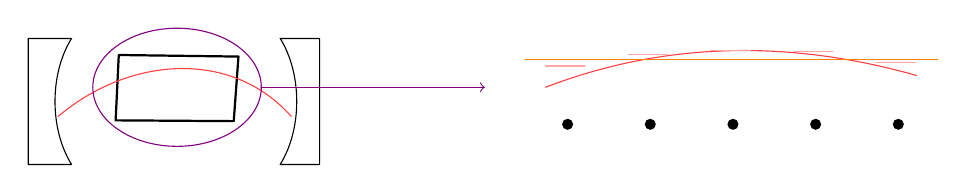
\begin{tikzpicture}[x=1cm,y=1cm,line cap=round,line join=round]
  \draw (0,0) -- (0,1.6) -- (.55,1.6)
        .. controls (.27,1.15) and (.27,.45) .. (.55,0) -- cycle;
  \draw (3.7,0) -- (3.7,1.6) -- (3.2,1.6)
        .. controls (3.48,1.15) and (3.48,.45) .. (3.2,0) -- cycle;
  \draw[thick] (1.11,.56) -- (1.15,1.39) -- (2.67,1.37) -- (2.61,.55) -- cycle;
  \draw[red!75] (.38,.61) .. controls (1.28,1.37) and (2.58,1.47) .. (3.34,.61);
  \draw[violet] (1.89,.98) ellipse (1.07 and .75);
  \draw[->,violet] (2.96,.98) -- (5.8,.98);
  \draw[red!75] (6.57,.98) .. controls (8.13,1.58) and (9.73,1.57) .. (11.28,1.13);
  \foreach \x/\y in {6.82/1.25,7.87/1.40,8.92/1.45,9.97/1.44,11.02/1.30}
      \draw[red!35] (\x-.25,\y) -- (\x+.25,\y);
  \draw[orange] (6.31,1.33) -- (11.55,1.33);
  \foreach \x in {6.85,7.90,8.95,10.00,11.05}
      \fill (\x,.51) circle (2pt);
\end{tikzpicture}
\end{center}

\textcolor{red!75}{\rule{1ex}{1ex}}\ exact: \(\vec A(\vec R)\),
\qquad
\textcolor{red!35}{\rule{1ex}{1ex}}\ first approx.:
\(\vec A(\vec R)=\vec A(\vec R_i,\vec R_0)\)

\textcolor{orange}{\rule{1ex}{1ex}}\ second approx.:
\(\vec A(\vec R)=\vec A\), i.e. constant over whole syst.

\item Eq. \paperref{paper:29}?

\item Why is \(L_{RR'}^{\mu\mu'}=0\) for one band Hubbard model?

\item In comparison to Li et al.: either Peierls phase or polarization
density but not both within one Hamiltonian
\end{itemize}

\end{document}
